\documentclass{40k}

\usepackage{pdflscape}
\usepackage[pdftex,hidelinks]{hyperref}

\usepackage[yyyymmdd]{datetime}

\newcommand{\checkbox}{\raisebox{-1pt}{\fbox{\hbox to 1em{\vbox to 1em{}}}}}

\newcommand{\letterbox}{\fbox{\hbox to 2em{\vbox to 32pt{}}}}

\newcommand{\scorebox}{\fbox{\hbox to 32pt{\vbox to 32pt{}}}}

\newcommand{\namebox}[1]{\fbox{\hbox to 92pt{\vbox to 64pt{\vfill\it #1}}}}

%%----------------------------------------------------------------------
%%----------------------------------------------------------------------
%%-- Story call-out

% We need to save the node
% Every append after command might be useful to have this code
\def\savelastnode{\pgfextra\edef\tmpA{\tikzlastnode}\endpgfextra}
\def\restorelastnode{\pgfextra\edef\tikzlastnode{\tmpA}\endpgfextra}
% Define box and box title style
\tikzstyle{borderbox} = [draw=black, very thick, fill=ltgray!20,
    rectangle, inner sep=15pt, inner ysep=12pt]
\tikzstyle{plainbox} = [draw=black, very thick, fill=white,
    rectangle, inner sep=15pt, inner ysep=12pt]
% rounded corners, 
\tikzstyle{fancytitle} =[fill=black, text=white]
\tikzstyle{club suit} = [append after command={%
    \savelastnode node[fancytitle,yshift=18pt] at (\tikzlastnode.south east)%
    {\includegraphics[width=1.5em]{icon-skull.pdf}}\restorelastnode }]
\tikzstyle{title} = [append after command={%
    \savelastnode node[fancytitle,right=10pt] at (\tikzlastnode.north west)%
    {\sc\fontfamily{ptm}\selectfont #1}\restorelastnode}]

\setlength{\fboxsep}{1pt}

\newenvironment{story}[2]{
\begin{realstory}{#1}{#2}{borderbox}
}
{
\end{realstory}
}

\newenvironment{realstory}[3]{
\noindent\hfil%
\begin{tikzpicture}%
\node [#3,club suit,title=#2] (box)\bgroup%
\vbox to #1 \bgroup\hbox to 0.8\linewidth \bgroup%
\begin{minipage}{0.8\linewidth}\it\fontfamily{ptm}\selectfont%
\noindent\ignorespaces%
}{%
\end{minipage}%
\egroup\egroup%
\egroup;%
\end{tikzpicture}%
}

\newenvironment{sidestory}[2]
{
\bigskip
\begin{story}{#1}{#2}
}
{
\end{story}
\smallskip
}
%%----------------------------------------------------------------------
%%----------------------------------------------------------------------

%%-- For cards
\pgfmathsetmacro{\cardroundingradius}{2mm}
\pgfmathsetmacro{\striproundingradius}{1mm}
\pgfmathsetmacro{\ruleheight}{0.1}
\pgfmathsetmacro{\stripwidth}{1.1}
\pgfmathsetmacro{\stripheight}{1.1}
\pgfmathsetmacro{\strippadding}{0.1}
\pgfmathsetmacro{\textpadding}{0.3}
\newcommand{\stripcolor}{black}
%%-------

\newcommand{\legacytitle}{CAMPAIGN LEGACY}
\newcommand{\legacystory}{Your must accomplish your quest!}
\newcommand{\legacymissiona}{Any}%
\newcommand{\legacyrolea}{Either}%
\newcommand{\legacymissionb}{Any}%
\newcommand{\legacyroleb}{Either}%
\newcommand{\legacymissionc}{Any}%
\newcommand{\legacyrolec}{Either}%
\newcommand{\legacygoal}{CRUSH FACE.}%
\newcommand{\legacybonus}{Hit yourself.}%

\pgfmathsetmacro{\legacycardwidth}{9.25}
\pgfmathsetmacro{\legacycardheight}{12.45}

\newcommand{\legacystripfontsize}{\huge}
\newcommand{\legacycaptionfontsize}{\LARGE}
\newcommand{\legacytextfontsize}{\large}

\newcommand{\legacystriptext}%
  {LEGACY: \legacytitle\hspace{0.5em}\rotatebox[origin=c]{-90}{\includegraphics[width=0.6cm]{icon-skull}}}


%%----------------------------------------------------------------------
%%----------------------------------------------------------------------
\newcommand{\resultstable}{%
\noindent\begin{minipage}{\linewidth}%
%\smallskip\centering\legacytextfontsize%
{\bf Twilight Missions:}\\
\centerline{\begin{tabular}{@{}C{1.3in}C{1in}c@{}}
  %{\bf Mission} & {\bf Role}&\\% & {\bf Victory}\\
  %\hline
  \legacymissiona & \legacyrolea & \ding{111}\\
  \legacymissionb & \legacyroleb & \ding{111}\\
  \legacymissionc & \legacyrolec & \ding{111}\\
  %\underline{\hspace{1.25in}} &  \underline{\hspace{0.8in}} & \ding{111}\\
\end{tabular}}%
\end{minipage}%
}


%%----------------------------------------------------------------------
%%----------------------------------------------------------------------
\newcommand{\drawlegacycard}{%
\begin{tikzpicture}%
  \clip (-0.05, -0.05) rectangle (\legacycardwidth+.05, \legacycardheight+.05);

  %%-- Draw the card back and outline
  \draw[rounded corners=\cardroundingradius,fill=white,draw=none] (0,0)
    rectangle (\legacycardwidth,\legacycardheight);
  \node[above left] at (\legacycardwidth+0.1, -0.1)
    {\includegraphics[width=3.5in]{background-skull}};
  \draw[rounded corners=\cardroundingradius] (0,0) rectangle
    (\legacycardwidth,\legacycardheight);

  %%-- Draw the side strip
  \fill[\stripcolor,rounded corners=\striproundingradius]
    (\strippadding,\strippadding) rectangle
    (\strippadding+\stripwidth,\legacycardheight-\strippadding)
    node[rotate=90,above left,white,font=\legacystripfontsize\fontfamily{ptm}\selectfont] {\raisebox{0pt}[15pt][3pt]{\vbox to -18pt{}} \legacystriptext};

  %%-- Draw the player info lines
    \node[text width=(\legacycardwidth-\strippadding-\stripwidth-2*\textpadding)*1cm,
          below right,inner sep=0] at
          (\strippadding+\stripwidth+\textpadding,\legacycardheight-\textpadding)
    {\legacytextfontsize%
      \raisebox{0pt}[26pt][0pt]{\begin{minipage}[b]{1.0\linewidth}\centering\it
          \legacystory
      \end{minipage}}

      %\bigskip
      %\centerline{\Large\sc\fontfamily{ptm}\selectfont --- Campaign ---}

      \bigskip
      \centerline{\resultstable}

      %\bigskip
      %\centerline{\Large\sc\fontfamily{ptm}\selectfont --- Cataclysm ---}

      \bigskip
      {\bf Cataclysm Objective:} \legacygoal

      \bigskip
      {\bf Legacy Bonus:} \legacybonus
    };

    \node[text width=(\legacycardwidth-\strippadding-\stripwidth-2*\textpadding)*1cm,
          above right,inner sep=0] at
          (\strippadding+\stripwidth+\textpadding,\strippadding)
    {\legacytextfontsize%
      \begin{tabular}{@{}ll}
        \textbf{Name:} &  \underline{\vbox to 18pt{}\hspace{2.125in}}\\
        %\textbf{Squad:} &  \underline{\vbox to 18pt{}\hspace{8.25cm}}\\
        %\textbf{Faction:} & \underline{\vbox to 18pt{}\hspace{8.25cm}}\\
        %\textbf{Alliance:} & \underline{\vbox to 18pt{}\hspace{8.25cm}}\\
      \end{tabular}
    };
\end{tikzpicture}
}


\newcommand{\legacycard}[9]{%
\renewcommand{\legacytitle}{#1}%
\renewcommand{\legacystory}{#2}%
\renewcommand{\legacymissiona}{#3}%
\renewcommand{\legacyrolea}{#4}%
\renewcommand{\legacymissionb}{#5}%
\renewcommand{\legacyroleb}{#6}%
\renewcommand{\legacymissionc}{#7}%
\renewcommand{\legacyrolec}{#8}%
\renewcommand{\legacygoal}{#9}%
\legacycardb%
}

\newcommand{\legacycardb}[1]{%
\renewcommand{\legacybonus}{#1}%
\drawlegacycard%
}


\begin{document}

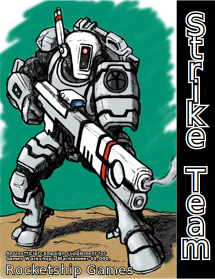
\includepdf[pages={1}]{art/cover/cover.pdf}

\pagetitle{Legacies}

%%----------------------------------------------------------------------
%%----------------------------------------------------------------------
\section{Introduction}

\begin{columns}

  \emph{Legacies} is an unofficial, team-oriented skirmish campaign
  for Games Workshop's \emph{Warhammer 40,000}.  Its core is a set of
  eight thematic missions designed for \emph{Recon Squad}, an
  unofficial skirmish variant of \emph{40k} similar to Games
  Workshop's \emph{Kill Team} rules.  Players field only a squad or
  two on a small board with dense terrain, and all their models act
  independently.  It's a very different \emph{40k} experience, focused
  on the heroics of regular grunts, without requiring you to learn new
  core rules.

  Those skirmishes are woven into a campaign here by a set of eight
  Legacies, specific missions the recon squads are striving to
  complete for their alliance.  The campaign climaxes in the
  Cataclysm, in which all the recon squads and some reinforcements
  fight alongside their alliance teammates in a final joint battle.

  \emph{Legacies} may be run either as a single full-day event or over
  several evenings.  Though the missions and legacies are thematic and
  storyful, \emph{Legacies} does not have its own setting, so that it
  can be easily adapted to one of your own making.  Other events are
  also easily connected before or after this campaign to form a larger
  narrative.  Notes are also included here on scoring \emph{Legacies}
  in a narrative tournament or league with individual prizes.

  Recon Squad rules are available here:

  \centerline{\url{rocketshipgames.com/40k/recon-squad/}}

\columnbreak
\noindent\fbox{\includegraphics[width=\linewidth]{art/recon-squad_cover.pdf}}
  
\subsection{Overview}

\emph{Legacies} is played as four rounds of Recon Squad skirmishes,
capturing small but pivotal incidents in a larger battle, followed by
a closing Cataclysm team game.

Each player's squad is working toward a legacy within the
greater conflict---

\begin{squishitemize}
\item \textbf{Bodyguards:} Fierce defenders of battlefield
  commanders;

\item \textbf{Excavators:} Daring explorers, technical experts, and
  artifact raiders;

\item \textbf{Headhunters:} Precision instruments of
  targeted violence;
%\end{squishitemize}

  % Following the events of \emph{The Debacle on Caldor IV} it has
  % become clear that the legendary \emph{Scythe of Unbound Light}
  % exists and is immeasurably important.  This discovery has spun the
  % maelstrom of conflict on Caldor IV to even dizzier velocities.
  % Unfortunately, the destruction of the planet is also now inevitable
  % with the Imperium having begun Exterminatus.  With every army
  % shattered and communication all but impossible, it is up to the
  % individual commanders and warriors in the field to rise to the
  % moment.  \emph{The Twilight of Caldor IV} plots the heroics of small
  % bands of warriors furiously moving into position to help their
  % alliance claim the relic before the end.


%\begin{squishitemize}
\item \textbf{Killers:} Shattered fighters disconnected from anything
  but bloodshed;

\item \textbf{Penetrators:} Sharpened blades able to break any
  armor or defense;

\item \textbf{Scouts:} Reckless adventurers reconnoitering the
  battlefield;

\item \textbf{Sentinels:} Implacable defenders and masters of \emph{ad
    hoc} fortifications;

\item \textbf{Warriors:} Hardened veterans that have been through
  everything.
\end{squishitemize}

Their path toward those legacies is defined by the missions they
tackle:

\smallskip\centerline{\begin{tabular}{C{1.5in}C{1.5in}}
\textbf{Ambush} & \textbf{Encirclement}\\
\textbf{Assassination} & \textbf{Excavation}\\
\textbf{Battlefield} & \textbf{Installation}\\
\textbf{Breakthrough} & \textbf{Skirmish}\\
\end{tabular}}

\smallskip%
Successes and failures at those challenges will define both the recon
squad's place in history, and their alliance's ability to win out in
the final Cataclysm.

\end{columns}

%%----------------------------------------------------------------------
%%----------------------------------------------------------------------
\clearpage
\pagetitle{Organization}

\begin{columns}

This section describes how to conduct a \emph{Legacies} campaign, and
is mostly intended for the organizer.

\missionheading{Schedule}

Recon Squad games can be easily run in about~60 minutes in an event
setting with boards pre-arranged and armies unpacked before the clock
starts for each round.  Generally matches take at most~90 minutes even
at a very casual pace with no preparation beforehand.  The Cataclysm
game can be comfortably played in~3--4 hours.  It's therefore feasible
to run \emph{Legacies} over either several evenings, or a single full
day.  A sample schedule for a single-day is as follows.

\bigskip
\centerline{\begin{tabular}{cl}
11:00	 	& Doors open\\
11:50	 	& Registration Closes\\
12:00	 	& Campaign Briefing \& Alliance Pairings\\
12:15	 	& Round 1\\
1:25	 	& Alliance Pairings\\
1:35	 	& Round 2\\
2:40	 	& Alliance Pairings\\
2:50	 	& Round 3\\
3:50	 	& Alliance Pairings\\
4:00	 	& Round 4\\
5:00	 	& Dinner Break\\
5:30	 	& The Cataclysm\\
9:30	 	& Campaign Outcome \& Prizes\\
\end{tabular}}

\missionheading{Alliances \& Story}

At the start of the campaign, the players are organized into two
alliances with an equal number of players.  In some groups this might
be faction specific, e.g., Chaos Daemons versus Eldar.  Generally
though an alliance will be comprised of several factions and can be
given a less specific title such as the Forces of Order, Legions of
Discord, or the Spoiler Horde.  How players are assigned alliances is
up to the organizer.  In a large event with mostly strangers and
tournament leanings it might be simply random.  In more
narrative-oriented and casual settings though, some attempt should be
made to take into account thematic cohesiveness as well as balanced
skill levels.

The concept behind the campaign is that each recon squad is a team of
veterans or other distinguished warriors tasked with several special
operations as part of a larger battle or war.  In the course of those
missions their paths eventually all cross, resulting in the larger
final battle.  Any specific background story is up to the organizer
and players, enabling a range of narratives with more or less detail.

\missionheading{Setup}

In advance of the campaign, players should at a minimum read the Recon
Squad rules and select their army list.  They should also be pointed
to the \emph{Legacies} Mission Pack, or this whole packet, in case
they wish to tailor their squad toward a particular legacy.

Preparing for the campaign is very simple.  For each of the two
alliances, print and cut apart enough sets of the~8 legacy cards at
the end of the Mission Pack section to have at least one card per
player.  Also print and cut apart enough sets of the~8 mission sheets
to have one for each match.  For a campaign with up to~16 players this
means making two sets of legacy cards and one set of mission sheets.

\missionheading{Legacies}

After being assigned an alliance, each player chooses a legacy.  No
legacy may be selected twice within an alliance until all legacies
have been chosen at least once, and so on if there are even more
players.  Otherwise the alliance members may discuss among themselves
how to divy up the legacies.  If there is any contention, either ask
the players in random order to choose, or randomly assign legacies.

Each legacy lists three Recon Squad Missions and gives a Cataclysm
Objective and Legacy Bonus.  To achieve their legacy, players must
accomplish the Cataclysm Objective in the final team battle.  If they
win at least two of the three Recon Squad Missions in the given role
of attacker, defender, or either, then they receive their Legacy Bonus
in the Cataclysm.

Players' chosen legacies, match results, and whether or not they are
succeeding at their missions are all public information throughout the
campaign.

\missionheading{Round Pairings}

Match pairings are made strategically by the alliances to help their
players achieve their legacy missions and further their collective
strategic goals.  Before each round, the alliances alternate
nominating one of their remaining unpaired players along with a
mission and role (attacker or defender).  The opposing alliance then
responds with a player for the match, who takes the other mission role
and chooses an unclaimed game board to play on.  This player must be
in the same or best similar win/draw/loss bracket as the nominated
player, unless the number of players is not great enough to make this
restriction without repeating match pairings.  In that case the later
rounds might require specific pairings to not have repeats.

For the first round, the initial alliance to put a player forward is
determined either randomly or based on the background story or the
outcomes of connected preceding events.  In subsequent rounds the
alliances alternate making the initial nomination.

Players should use the checkboxes on their legacy cards to record
victories toward the Recon Squad Mission requirements, in addition to
the organizer keeping track.  It does not matter if the player was
nominated or the responding opponent, and they do not have to complete
the missions in any order.  In order to get their Legacy Bonus in the
Cataclysm they simply have to win each mission in the required role at
some point in the campaign.  Similarly, a player can attempt a mission
and role pair multiple times.  However, no advantage is gained by
winning the same mission and role pair multiple times.

\end{columns}

%%----------------------------------------------------------------------
%%----------------------------------------------------------------------
\vbox to 0pt{}
\vfill
\noindent
\begin{minipage}[t]{1.0\linewidth}\centering%
\rowcolors{2}{gray!12}{white}\setlength{\tabcolsep}{3pt}%
\resizebox{\linewidth}{!}{\begin{tabular}{|l|C{1in}|C{1in}|C{1in}|C{1in}|C{1in}|C{1in}|C{1in}|C{1in}|}
\hline
\rowcolor{gray!25} {\bf Mission}       
                    & {\bf Bodyguards}  & {\bf Excavators}& {\bf Headhunters}   & {\bf Killers}   & {\bf Penetrators}&{\bf Scouts}   & {\bf Sentinels} & {\bf Warriors}\\
\hline
\hline
{\bf Ambush}        & Defender          & Either         & Attacker             &                 &                 & Attacker       &                 &               \\
{\bf Assassination} & Defender          &                & Attacker             &                 & Attacker        &                &                 &               \\
{\bf Battlefield}   &                   &                &                      & Either          &                 &                &                 & Either        \\
{\bf Breakthrough}  & Attacker          &                &                      &                 & Attacker        &                & Defender        &               \\
{\bf Encirclement}  &                   &                &                      & Attacker        &                 &                & Defender        & Defender      \\
{\bf Excavation}    &                   & Either         & Either               &                 &                 & Either         &                 &               \\
{\bf Installation}  &                   & Either         &                      &                 & Attacker        &                & Defender        &               \\
{\bf Skirmish}      &                   &                &                      & Either          &                 & Either         &                 & Either        \\
\hline
\end{tabular}}

\small\it\smallskip
Recon Squad mission and role requirements for the legacies.
\end{minipage}
\vfill


%%----------------------------------------------------------------------
%%----------------------------------------------------------------------
\clearpage

\begin{columns}


\end{columns}


%%----------------------------------------------------------------------
%%----------------------------------------------------------------------
\clearpage
\pagetitle{The Twilight: Mission Pack}


All of the missions are played on a~4'x4' table.

The variable game length rule is used in all missions unless noted otherwise.

  Roll a~D6 before any
deployment.  Night Fighting is in effect for Turn~1 on a~4+; on a~1
or~2 it takes effect on Turn~5 and thereafter.

The winner of a~D6 roll off decides to deploy first or second.  After
both players deploy, the player that deployed first chooses to play
first or second.  The player to go second may attempt to Seize the
Initiative.


A major victory is worth 10 points to the winner and 0 to the loser.
Victory is 7 and 3
Draw is 5 and 5

Plus the two bonus points.

Better victories trump others, e.g., meeting the conditions for a
major victory trumps the conditions for a minor victory.

Missions to be specified in more detail...

\missionheading{Ambush}

The Defender is given an AV10/10/10 HP2 truck with 5 embarked NPCs
with sub-Guardsman stats.  The truck takes dangerous terrain tests on
a 2+ and always takes a dangerous terrain test if it moves flat out.
The truck starts at one end of the board and it or the NPCs must make
it to the far edge.  The Attacker Outflanks.


\missionheading{Assassination}

An NPC with Guardsman-ish stats is placed in control of the Defender,
who loses if it dies.


\missionheading{Battlefield}

Kill points with Dawn of War setup.


\missionheading{Breakthrough}

Attacker has to break into the defender's deployment zone.


\missionheading{Encirclement}

Kill points with the defender starting at the center of the table and
the attacker all around.


\missionheading{Excavation}

Similar to the scouring, several objectives of randomized value are
randomly placed inside a square at table center.  The defender starts
deployed in that square, the attacker is around the edges.


\missionheading{Installation}

A single objective is put forward slightly from the defenders leading
edge, inside an AV11 HP3 Small building.  The defender wins if they
hold that objective.  Otherwise the attacker wins.


\missionheading{Skirmish}

The basic mission from the Recon Squad packet: Vanguard and three objectives.


\pagestyle{empty}

%%----------------------------------------------------------------------
%%----------------------------------------------------------------------
\clearpage
\pagetitle{Missions}

\begin{columns}
  
  Army rules, legacies, and missions for the campaign are in this
  section and should be read by all players.

\missionheading{Campaign}

The campaign consists of four rounds of Recon Squad skirmish matches,
followed by the Cataclysm, a climactic team battle.  Army construction
and gameplay rules for the Recon Squad rounds are here:

\smallskip
\centerline{\url{http://rocketshipgames.com/40k/recon-squad/}}

\smallskip%
The Cataclysm uses standard 40k gameplay rules except as described in
this packet.

At the start of the campaign, players join an alliance and choose a
legacy.  Legacies cannot be repeated within an alliance until all have
been chosen.  In each of the Recon Squad rounds, the alliances
alternate choosing missions from those in this section.

\missionheading{Army Construction}

Each player must prepare two lists:

\begin{itemize}\shortlist
  \item {\bf Recon Squad:} For the skirmish missions;
  \item {\bf Cataclysm:} For the climactic final team battle.
\end{itemize}

Recon Squad lists are selected to at most~200 points, following the
rules in that packet.  Cataclysm lists are selected to at most~500
points by these rules:

  \begin{itemize}\shortlist
  \item Each player's Recon Squad list must be included in their
    Cataclysm list in its entirety.

  \item Additional units and models (with wargear and upgrades) may be
    added to the Recon Squad Detachment.  However, the original models
    may not receive new wargear or upgrades.

  \item A single Cataclysm Reinforcements Detachment may be added to
    the army, with a force organization of~0--1 HQ,~1--3 Troop,~0--1
    Elite,~0--1 Fast Attack,~0--1 Heavy Support, and~0--1
    Fortification.  All its units must be chosen from a single
    faction, but that may be a different faction from the Recon Squad
    Detachment.

  \item No models with more than~3 wounds/hull points.

  \item No vehicles with total armor (front + side + rear) of more
    than~33.

  \item No models with both a~2+ Armor and~3+ Invulnerable save or
    better are permitted.

  \item No flyers, flying monstrous creatures, superheavy vehicles,
    gargantuan creatures, or mighty bulwarks are permitted.

  \item No psykers of mastery level~2 or greater.

  \item No unique independent characters or unique wargear is
    permitted.
  \end{itemize}

\missionheading{Recon Squad Mission Rules}
The Recon Squad missions use the following rules:

\begin{itemize}\shortlist
\item Matches are played on~4''x4'' tables.

\item The Variable Game Length rule applies.

\item If either player wishes the game to be a night fight, roll a~D6
  before any deployment begins. Night Fighting is in effect (all units
  have Stealth) for game turn~1 on a~4+; on a result of~1 Night
  Fighting takes effect for turn~5 and thereafter.

\item Unless specifically noted otherwise by the mission, deployment
  and turn order follows the standard rules: The winner of a D6 roll
  off decides to deploy first or second. After both players deploy,
  the player that deployed first chooses to play first or second. The
  player to go second may attempt to Seize the Initiative.

% Match results are worth the following campaign points. mostly relevant just to the larger narrative: A major victory outcome is worth 10 campaign points to the winner and 0 to the not-winner. Minor victory outcomes award 7 and 3 campaign points respectively. Draws award 5 campaign points to each player. Two additional bonus points are available in each mission, and if achieved are awarded regardless of victory or not. Better victories trump other results, e.g., meeting the conditions for a major victory renders the minor victory and draw conditions irrelevant.
\end{itemize}

\end{columns}

%%----------------------------------------------------------------------
%%----------------------------------------------------------------------

\vfill
\noindent
\begin{minipage}[t]{1.0\linewidth}\centering%
\rowcolors{2}{gray!12}{white}\setlength{\tabcolsep}{3pt}%
\resizebox{\linewidth}{!}{\begin{tabular}{|l|C{1in}|C{1in}|C{1in}|C{1in}|C{1in}|C{1in}|C{1in}|C{1in}|}
\hline
\rowcolor{gray!25} {\bf Mission}       
                    & {\bf Bodyguards}  & {\bf Excavators}& {\bf Headhunters}   & {\bf Killers}   & {\bf Penetrators}&{\bf Scouts}   & {\bf Sentinels} & {\bf Warriors}\\
\hline
\hline
{\bf Ambush}        & Defender          & Either         & Attacker             &                 &                 & Attacker       &                 &               \\
{\bf Assassination} & Defender          &                & Attacker             &                 & Attacker        &                &                 &               \\
{\bf Battlefield}   &                   &                &                      & Either          &                 &                &                 & Either        \\
{\bf Breakthrough}  & Attacker          &                &                      &                 & Attacker        &                & Defender        &               \\
{\bf Encirclement}  &                   &                &                      & Attacker        &                 &                & Defender        & Defender      \\
{\bf Excavation}    &                   & Either         & Either               &                 &                 & Either         &                 &               \\
{\bf Installation}  &                   & Either         &                      &                 & Attacker        &                & Defender        &               \\
{\bf Skirmish}      &                   &                &                      & Either          &                 & Either         &                 & Either        \\
\hline
\end{tabular}}

\small\it\smallskip
Recon Squad mission and role requirements for the legacies.
\end{minipage}

\clearpage
\thispagestyle{empty}
\squelchbackground

\noindent%
\legacycard{BODYGUARDS}%
{Our lives for you, my liege.\\~}%
{Ambush}%
{Defender}%
{Assassination}%
{Defender}%
{Breakthrough}%
{Attacker}%
{After all deployment, publicly pledge to defend one of your alliance's
  warlords other than your own.  You succeed if that warlord is on the battlefield at game end (i.e., survived and not embarked).}%
{Whenever your pledged warlord
loses a wound, on a~D6 of ~2+ the loss may be cancelled by one of your non-Vehicle
models within~3'' taking a mortal wound instead.}
%%
\hfill
%%
\legacycard{EXCAVATORS}%
{Get it into the crates,\\quickly, this is ours!}%
{Ambush}%
{Either}%
{Excavation}%
{Either}%
{Installation}%
{Either}%
{After all deployment ends, secretly select an objective marker wholly
  outside your deployment zone.  You succeed if you control that objective marker at game
  end.}%
{Any single non-Vehicle model of yours that starts the movement
  phase in contact with \emph{any} marker may move it up to~6'' with
  the model's movement.  The marker cannot leave the table, including to embark a Transport.}


\noindent%
\legacycard{HEADHUNTERS}%
{Death comes for us all.\\We come for you.}%
{Ambush}%
{Attacker}%
{Assassination}%
{Attacker}%
{Excavation}%
{Either}%
{After all deployment, secretly select one of the opposing warlords.
  You succeed if that warlord is not in play at game end.}%
{Your non-Vehicle models may shoot at that warlord regardless of
it being the closest enemy or not.}
%%
\hfill
%%
\legacycard{KILLERS}%
{Kill.  Maim.  Burn.\\~}%
{Battlefield}%
{Either}%
{Encirclement}%
{Attacker}%
{Skirmish}%
{Either}%
{After all deployment, publicly declare a crusade against an opposing
  player.  You succeed at game end if at most 25\% of that player's
  starting army points remain in play (i.e., they have at most 125pts).}%
{In the fight phase your non-Vehicle models receive a~+1 to hit against that opponent's units.}

\pagebreak
\thispagestyle{empty}

\noindent%
\legacycard{PENETRATORS}%
{Everything has a weak spot.\\~}%
{Assassination}%
{Attacker}%
{Breakthrough}%
{Attacker}%
{Installation}%
{Attacker}%
{At game end your units control at least one primary objective marker
  in the opposing deployment zone.}%
{After all deployment ends you may ruin a piece of terrain or opposing fortification,
reducing any associated cover by~1 (to~+0 at worst).}
%%
\hfill
%%
\legacycard{SCOUTS}%
{Let's go, on the move!\\~}%
{Ambush}%
{Attacker}%
{Excavation}%
{Either}%
{Skirmish}%
{Either}%
{Control at least three different objective
  markers outside your deployment zone at the end of any of your turns over the course of the game (not necessarily
  simultaneously).}%
% {At the end of each of your turns except the first, make a note for
%   each primary objective marker you control outside your deployment
%   zone which you have not previously controlled.  You succeed if you
%   note at least three.}%
%
{Your non-Vehicle units may deploy on maneuver
instead of on the battlefield.  At the end of any of your Movement phases they may be set up anywhere on the battlefield wholly within~6'' of a battlefield edge and more than~9'' from all enemy models.}

\vfill


\noindent%
\legacycard{SENTINELS}%
{None shall pass.\\~}%
{Breakthrough}%
{Defender}%
{Encirclement}%
{Defender}%
{Installation}%
{Defender}%
{At game end your units control all the primary objective markers that
  began in your deployment zone.}%
{After all deployment ends you may bolster a piece of terrain or a
  fortification in your deployment zone, improving any associated
  cover bonus by~1, to~+2 at best.}
%%
\hfill
%%
\legacycard{WARRIORS}%
{This isn't over.\\This will never be over.}%
{Battlefield}%
{Either}%
{Encirclement}%
{Defender}%
{Skirmish}%
{Either}%
{There are no enemy models in your deployment zone at
  game end.}%
{Whenever one of your non-Vehicle models loses a wound, the loss is cancelled
on a~D6 of~6+. If the model already had such a rule then the loss is cancelled on a~5+.}


\clearpage
\restorebackground



\newcommand{\scoringbox}[5]{%
\vfill%
\vspace{9pt}%
\noindent\vbox{%
\noindent\vbox to -4pt{\noindent\hfill\Large\bf\sc\fontfamily{ptm}\selectfont Scoring\vbox{}}\\
%
{\fbox{\vbox{\small%
\setlength{\tabcolsep}{2pt}%
\noindent\begin{tabularx}{\linewidth}{cccX}
  \hbox to 1.25em{\rotatebox{45}{\small\bf Attacker}}&
  \hbox to 1.25em{\rotatebox{45}{\small\bf Defender}}&
  &
  \multicolumn{1}{c}{\footnotesize\bf Condition}
\\
  \hline
%
  \rescheck&\rescheck& & {\bf Major Victory:} #1\\
%
  \rescheck&\rescheck& &
  {\bf Minor Victory:} #2\\
%
\rescheck&\rescheck& &
{\bf Draw:} #3\\
\hline \rescheck&\rescheck& &
{\bf Bonus Point:} #4\\
\rescheck&\rescheck& &
{\bf Bonus Point:} #5\\
\end{tabularx}%
}}}}%
}

\clearpage
\squelchbackground

%%----------------------------------------------------------------------
%%----------------------------------------------------------------------
\missiontitle{Mission: Ambush}

\begin{columns}

A supply convoy is moving through the area.

  {\bf Attacker:} You \emph{need} those supplies.

  {\bf Defender:} The supplies must get through.

\missionheading{The Battlefield}%

The winner of a~D6 roll off chooses a table edge and the other player
takes the opposite.  The defender's deployment zone is the~12'' strip
along their table edge.  All of the attacker's units gain Outflank and
must be placed in reserve, except Infiltrators which may deploy as
usual.  At the start of their deployment, the defender gains a convoy
vehicle for their army.

%Place a small vehicle with its forward edge~6'' from the
%defender's edge and center 24'' from the sides.

\missionheading{Mission Rules}%

%The attacker plays first.  The defender may not Seize the Initiative.

Half of the attacker's army by the number of models, rounding up,
arrives from reserve on Turn~1.  The remainder arrive from reserve as
usual.

The convoy vehicle has armor~11/11/10,~3 hull points, and may not move
Flat Out.  It ignores all results on the Vehicle Damage table, only
losing the hull point when damage is incurred.  On a failed dangerous
terrain test it loses a hull point and cannot move further that phase
but is not immobilized.  The vehicle, or its wreck, also acts as an
objective marker.  While the vehicle is not destroyed, the defender
controls it by default if there are no attacker models within 3''.

% At game start it is controlled by the
% defender.  Either player may take control of the vehicle by ending
% their turn with they alone having an unengaged model in base contact.
% Models do not need to remain in contact to keep control.

%If
%immobilized, the vehicle self-repairs and removes that damage result
%on a~D6 of~4+ at the start of the defender's movement phase.

%At game end, victory points are earned as follows:
%
%\begin{squishitemize}
%\item Each player gets~2 victory points for each~12'' the vehicle is
%  from their edge, rounding down.
%
%\item At least 50\% of the opponent's army by points value or number
%  of models are casualties: +2
%
%\item All of the opponent's models have been removed as casualties: +1
%\end{squishitemize}

%\vspace*{-17pt}

\scoringbox%
{Attacker if the vehicle is destroyed and they control its wreck.
  Defender if the vehicle or its wreck is within 12'' of the attacker
  table edge and they control it.}%
{Attacker if the vehicle is not destroyed but they control it.
  Defender if they control the vehicle or its wreck, but it is not
  within 12'' of the attacker table edge.}%
{The vehicle or its wreck is contested.}%
{Opponent's leader is a casualty.}%
{Player's leader survives.}

\end{columns}

%%----------------------------------------------------------------------
%%----------------------------------------------------------------------
\missiontitle{Mission: Assassination}

\begin{columns}

  A VIP is touring the frontlines, their mission unknown.

  {\bf Attacker:} The VIP must be slain.

  {\bf Defender:} The VIP must be defended at all cost.

\missionheading{The Battlefield}%

Deployment zones are 12'' from opposing table edges.  The winner of
a~D6 roll off chooses a side and the other player takes the opposite.
Before deploying, the defender's army gains a VIP model.

Place~3 objective markers at~12'' intervals along the centerline 24''
from both player table edges.

\missionheading{Mission Rules}%

The VIP is an infantry character with WS2 BS2 S3 T3 W3 I2 A1 LD8, a~2+
armour save and ~4+ invulnerable, Eternal Warrior, Fearless, and a
laspistol.

At game end, each objective marker is worth~1 victory point.  The
defender gets~2 victory points for each wound remaining on the VIP.
The attacker gets~2 victory points for each wound lost by it.

\scoringbox%
{Player has at least twice as many victory points as their opponent.}%
{Player has more victory points.}%
{Players have equial victory points.}%
{Opponent's leader is a casualty.}%
{Player has a model in opponent's deployment zone.}

\end{columns}

%%----------------------------------------------------------------------
%%----------------------------------------------------------------------
\clearpage
\section{Mission: Battlefield}


The war grinds on interminably, all notion of battle lines lost in
confusion and exhaustion.

\begin{squishitemize}
\item \textbf{Attacker} and \textbf{Defender} roles are identical in
  this mission and have no effect in-game.
\end{squishitemize}

\subsection{\bf The Battlefield}%

The winner of a~D6 roll off chooses a table corner.  Their deployment
zone is the quarter circles of all points within~12'' of that corner
as well as the \emph{diagonally} opposite corner.  The other player's
deployment zone is the~12'' quarter circles from the other corners.

Place a single objective marker at table center.

% \vfill
% \vbox to 0pt{}
% \columnbreak

\subsection{\bf Mission Rules}%

At game end, victory points are earned as follows:

\begin{squishitemize}
\item At least~3 of your opponent's models have been removed as
  casualties: +2

\item At least 50\% of your opponent's army by points or models are
  casualties: +3

\item The total number of wounds lost by your opponent is more than
  you: +1

\item All of your opponent's models have been removed as casualties:
  +1
\end{squishitemize}

\vfill

\scoringbox%
{Player has at least twice as many victory points as their opponent.}%
{Player has more victory points.}%
{Players have equial victory points.}%
{Opponent's leader is a casualty.}%
{Controls the objective marker.}

%%----------------------------------------------------------------------
%%----------------------------------------------------------------------
\missiontitle{Mission: Breakthrough}

\begin{columns}

  Opposing forces thrust and counter-thrust to break up or hold
  battlefield positions.

{\bf Attacker:} You must pierce the enemy's lines.

{\bf Defender:} Hold your ground.

\missionheading{The Battlefield}%

The winner of a~D6 roll off chooses a table edge and the other player
takes the opposite.  Deployment zones are~12'' from the players'
respective edges.

% , but the defender's models must all be placed at
% least~6'' from their player table edge.

% Place~4 objective markers,~6'' and~18'' from the two side edges and
% all 3'' from the defender table edge.

\missionheading{Mission Rules}%

At game end, victory points are earned as follows:

\begin{squishitemize}
\item The defender earns~2 victory points for each quarter of their
  army by number of models that has not been removed as a casualty,
  rounding down (i.e., less than~25\% is worth no points).

\item The defender earns~1 victory point if no attacker models are in
  the defender's table half.

\item The attacker earns~1 victory point for each quarter of their
  army by models that has not been removed as a casualty, rounding
  down.

\item The attacker earns~1 victory point for each quarter of their
  starting army by models that is at least partially within 6'' of the
  defender table edge, rounding up (i.e., having at least~1 model
  within 6'' of the defender edge is worth a point).

\end{squishitemize}

% \vfill
% \vbox to 0pt{}
% \columnbreak

\scoringbox%
{Player has at least twice as many victory points as their opponent.}%
{Player has more victory points.}%
{Players have equial victory points.}%
{Opponent's leader is a casualty.}%
{Leader is within 12'' of opponent's player table edge.}

% \scoringbox%
% {Attacker if they control at least~3 objective markers.  Defender if
% the attacker controls no objective markers.}%
% {Attacker if they control at least~1 objective marker.}%
% {Otherwise.}%
% {Opponent's leader is a casualty.}%
% {Player's leader is the closest model to the defender's table edge.}

% \scoringbox%
% {Attacker if at least~50\% of their starting army by number of models
%   is at least partially within~6'' of the defender's table edge.
%   Defender if attacker has no models within~6'' of the defender's
%   table edge.}%
% {Attacker if more than~25\% of their starting army by number of models
%   is at least partially within~6'' of the defender's table edge.
%   Defender if attacker has at most 25\% of their starting army by
%   points value or number of models within~6'' of the defender's table
%   edge.}%
% {Otherwise.}%
% {Opponent's leader is a casualty.}%
% {Player's leader is the closest model to the defender's table edge.}

\end{columns}

%%----------------------------------------------------------------------
%%----------------------------------------------------------------------
\missiontitle{Mission: Encirclement}

\begin{columns}

  A small force has been outmaneuvered and surrounded in a tight
  pocket of the battle.

{\bf Attacker:} Crush them.

{\bf Defender:} Survive.

\missionheading{The Battlefield}%

The winner of a~D6 roll off chooses a table edge and the other player
takes the opposite.  The attacker's deployment zone is~6'' from
\emph{both} player table edges.  The defender's deployment zone is
the~12'' center strip~18'' from both player table edges.


\missionheading{Mission Rules}%

At game end, victory points are earned as follows:

\begin{squishitemize}
\item At least~3 of your opponent's models have been removed as
  casualties: +2

\item At least 50\% of your opponent's army by points value or number
  of models are casualties: +3

\item The total number of wounds lost as a casualty by your opponent
  is more than you: +1

\item All of your opponent's models have been removed as casualties:
  +1
\end{squishitemize}

\vspace*{-2pt}

\scoringbox%
{Player has at least twice as many victory points as their opponent.}%
{Player has more victory points.x}%
{Players have equial victory points.}%
{Opponent's leader is a casualty.}%
{Player has a model in each table quadrant, at least~3'' from table center.}

\end{columns}

%%----------------------------------------------------------------------
%%----------------------------------------------------------------------
\missiontitle{Mission: Excavation}

\begin{columns}

  An important relic was uncovered by an excavation team just before
  they were forced to abandon the site by the encroaching battle.  It
  must be retrieved!

  \textbf{Attacker} and \textbf{Defender} roles are identical in this
  mission and have no effect in-game.

\missionheading{The Battlefield}%

Deployment zones are 12'' from opposing table edges.  The winner of
a~D6 roll off chooses a side and the other player takes the opposite.

Place a primary objective marker at the center of the table and
secondary objective markers at the center of each table quadrant.


\missionheading{Mission Rules}%

Any model that starts the movement phase in base to base contact with
the \emph{primary} objective marker while no enemy models are in base
to base contact with it may move the marker with itself up to a total
of 6'' in the movement phase, ending in contact with the model.  The
marker cannot leave the table or embark.

%\columnbreak

At game end, control of the primary objective is worth~3 victory
points while each secondary objective is worth~1 victory point.

\scoringbox%
{Player controls the primary objective and has more victory points.}%
{Player has more victory points.}%
{Players have equal victory points.}%
{Opponent's leader is a casualty.}%
{The primary objective marker is fully within your deployment zone.}

\end{columns}

%%----------------------------------------------------------------------
%%----------------------------------------------------------------------
\missiontitle{Mission: Installation}

\begin{columns}

  A critical outpost, command center, supply warehouse, or temple has
  come under siege!

{\bf Attacker:} You must destroy it and control the site.

{\bf Defender:} You must protect the installation.

\missionheading{The Battlefield}%

Deployment zones are 12'' from opposing table edges, with the attacker
choosing and the defender taking the opposite.  Before their
deployment, the defender's army gains a small building fortification.

\missionheading{Mission Rules}%

The defender deploys first but the attacker plays first.  Seize the
Initiative applies.  The building cannot be placed within~6'' of any
table edge.  It has armor~11 on each facing,~3 hull points, a
transport capacity of~5, battlements on top, and access points on the
sides and back.  If the building is destroyed, its ruins or crater are
treated as an objective marker.

% Control of the building or its ruins is determined as an objective
% marker, including embarked models.


\columnbreak

\scoringbox%
{Attacker if the building is destroyed and they control the wreckage.
  Defender if the building is not destroyed and they control it.}%
{Attacker if the building is destroyed but contested, or intact but
  they control it.  Defender if the building is destroyed but they
  control the wreckage.}%
{\emph{There is no middle ground in this mission.}}%
{Opponent's leader is a casualty.}%
{Less than 25\% of opponent's starting army remains, by
  number of models.}

\end{columns}

%%----------------------------------------------------------------------
%%----------------------------------------------------------------------
\missiontitle*{Mission: Skirmish}

\begin{columns}

  Vanguards patrolling the outskirts of their main forces have crashed
  into each other---contact is made!

  \textbf{Attacker} and \textbf{Defender} roles are identical in this
  mission and have no effect in-game.

\missionheading{The Battlefield}%

% A variety of ruins, woods, and other terrain should be placed to
% cover a quarter to a half of the board evenly and roughly
% symmetrically.

Deployment zones are diagonal table corners, up to~12'' from the
centerline between them.  Roll off to determine who chooses a corner
and their player table edge, the other player taking the opposite.

Place objective markers at the center of the table and the centers of
the two table quadrants opposite the deployment zone corners.

\columnbreak

\scoringbox
{Player controls at least
  two more objective markers than opponent, or opponent has been
  completely eliminated.}
{Player controls at least one more
                       objective marker than opponent.}
{Players control equal objective markers.}
{Opponent's leader is a casualty.}
{Player has at least one model within 12'' of each table corner.}

\end{columns}
%

\clearpage
\restorebackground


%%----------------------------------------------------------------------
%%----------------------------------------------------------------------
\missiontitle{The Cataclysm}

\begin{columns}
  
  All of the recon squads have crossed paths as they fight toward
  their final missions!

  The alliance with fewer total points earned in the Recon Squad
  matches is considered the {\bf Defender}, and the other alliance the
  {\bf Attacker}.

  \missionheading{Heroes}

  Before the game begins, the specialists in each player's recon squad
  are elevated to be independent characters.  Each leader additionally
  gains~1 Wound, is considered to be an HQ unit, and is their player's
  warlord.  The warlords receive a warlord trait as usual, and players
  may reroll randomly chosen traits.

  Before any deployment, each alliance declares one of their warlords
  to be their warmaster.

  \missionheading{The Battlefield}

  Deployment zones are the areas up to~12'' from the long table edges
  and along their length (Dawn of War).  The defender chooses a zone
  and the attacker takes the other, both taking the long edge of their
  zone as their player table edge.  The defender then places~3 primary
  objective markers in its deployment zone, after which the attacker
  places~3 in its zone.

  After all deployment (before any Scout redeployments), each player
  places a secondary objective marker, alternating sides beginning
  with the defender.

  The defender chooses to play first or second.

  \missionheading{Mission Rules}

  Night Fighting, Seize the Initiative, and Reserves all apply as in
  the standard Eternal War missions.  The Cataclysm ends after game
  turn~5.

  \missionheading{Scoring}

  Objective markers are scored after each game turn: Primaries award
  the current turn number in victory points, while secondaries award~1
  victory point.

  % \begin{itemize}
  % \item Primaries award the current turn number in victory points;
  % \item Secondaries award~1 victory point.
  % \end{itemize}

  Alliances gain~2 victory points if the opposing warmaster is removed
  as a casualty, and~1 victory point for each other opposing warlord
  eliminated.

  First Blood and Linebreaker both apply as in the standard Eternal
  War missions.

  % The first unit (including single models) to be removed in its
  % entirety for any reason yields~1 victory point to the opposing
  % alliance for first blood.  If an alliance has any scoring units in
  % its opponent's deployment zone at game end then it scores~1 victory
  % point for linebreaker.

  Whichever alliance scores the most victory points wins a tactical
  victory in the Cataclysm, while the alliance that has more players
  achieve their legacy objectives wins a strategic victory.

\end{columns}


\end{document}
